\documentclass{llncs}

\usepackage{amssymb}
\usepackage{amsmath}
\usepackage{url}
\usepackage{graphics}
\usepackage{graphicx}
\usepackage[all]{xy}
\usepackage{float}
\usepackage{listings}
\usepackage{lipsum}

\usepackage[ruled,vlined]{algorithm2e}
\usepackage{alltt}
\urldef{\mailsa}\path|pat@dcs.gla.ac.uk|
\newcommand{\keywords}[1]{\par\addvspace\baselineskip
\noindent\keywordname\enspace\ignorespaces#1}
\newlength{\halftextwidth}
\setlength{\halftextwidth}{0.47\textwidth}
\usepackage{multicol}
\usepackage{listings}
\usepackage{url}
\usepackage{coffee2}
%\usepackage{amsthm}
%\newtheorem*{definition}{Definition}#
\usepackage{amsopn}

\newcommand{\match}{\mathit{match}}
\newcommand{\timeSlot}{\mathit{timeSlot}}
\newcommand{\state}{\mathit{state}}
\newcommand{\change}{\mathit{change}}
\newcommand{\totalChange}{\mathit{totalChange}}
\newcommand{\totalBoatChanges}{\mathit{totalBoatChanges}}
\newcommand{\modMatch}{\mathit{modMatch}}
\newcommand{\position}{\mathit{position}}
\newcommand{\imbalance}{\mathit{imbalance}}
\newcommand{\maxImbalance}{\mathit{maxImbalance}}

\newcommand{\START}{\textnormal{\textsc{Start}}}
\newcommand{\FIRST}{\textnormal{\textsc{First}}}
\newcommand{\MID}{\textnormal{\textsc{Mid}}}
\newcommand{\LAST}{\textnormal{\textsc{Last}}}
\newcommand{\END}{\textnormal{\textsc{End}}}
\newcommand{\BYE}{\textnormal{\textsc{Bye}}}

\newcommand{\eachOccursExactlyOnce}{\mathrm{eachOccursExactlyOnce}}
\newcommand{\allDifferent}{\mathrm{allDifferent}}

\pagestyle{plain}
\begin{document}

\title{Constructing Sailing Match Race Schedules: Round Robin Pairing Lists}
\titlerunning{Match Race Scheduling}
%\toctitle{}
\author{Craig MacDonald \and Ciaran McCreesh \and Alice Miller \and Patrick Prosser}
\institute{University of Glasgow, Glasgow, Scotland \\ \email{patrick.prosser@glasgow.ac.uk}}
\authorrunning{MacDonald, McCreesh, Miller, Prosser}
\maketitle

\begin{abstract} 
The quick brown duck jumped over the lazy pig. The quick brown duck jumped over the lazy dog. The quick brown duck jumped over the lazy dog. The quick brown duck jumped over the lazy dog.
\end{abstract}

\section{Introduction}
\coffee{1}

\section{Problem Definition: round robin pairing lists}
In the ISAF International Umpire's and Match Racing Manual \cite{isaf}, section
M.2 Recommended Criteria for Round Robin Pairing Lists, the following criteria
are given:

\begin{enumerate}
\item Each skipper sails against each other skipper once.
\item When there is an even number of flights, each skipper has the same number
    of port and starboard assignments.
\item When there is an odd number of flights, the first half of the skippers
    will have one more starboard assignment.
\item No skipper in the last match of a flight should be in the first match of
    the next flight.
\item No skipper should have more than two consecutive port or starboard
    assignments.
\item Each skipper should be assigned to match 1, match 2, etc. in a flight as
    equally as possible.
\item In flights with five or more matches no skipper should be in the
    next-to-last match in a flight and then in the first match of the next
    flight.
\item If possible, a skipper should be starboard when meeting the nearest
    lowest ranked skipper (i.e. \#1 will be starboard against \#2, \#3 will be
    starboard against \#4).
\item Close ranked skippers meet in the last flight.
\item Minimize the number of boat changes.
\item Skippers in the last match of a flight do not change boats.
\item Skippers in new boats do not sail in the first match of the next flight.
\item Skippers have a reasonable sequence of matches and blanks.
\end{enumerate}

Note that criteria 10, 11 and 12 only apply when there are fewer boats than
skippers.

\section{The Constraint Models}

The schedules are produced in four stages. The first stage produces a schedule
that respects criteria 1, 4, 11 and 12, and minimises criteria 10 (boat
changes). The second stage constructs a schedule that respects criteria 1, 4,
11, 12 (again), has criteria 10 as a hard constraint generated from first
stage, and minimises criteria 6 (balance). This results in a schedule that
attempts to minimise boat changes \emph{and} balance. The third stage satisfies
criteria 9, and is a simple translation of the schedule produced in stage 2.
The final stage, orients skippers within matches to address criteria 2, 3, 5
and 8.

We now describe the constraint models and processes used in each stage. In the
text below we assume there are $n$ skippers and $b$ boats, with $m = b/2$
matches in a flight. In total there are $t = n(n-1)/2$ matches and $f = \lceil
n(n-1)/m  \rceil$ flights. We use the schedule in Table~\ref{tab1}, for 7
skippers and 6 boats, to help illustrate the constraint models. Our
descriptions of the models omit some minor details, however the models are
available to download\footnote{?? give us a link to the models}.

\begin{table}[tb]
\begin{center}
\begin{tabular}{cc} \\
flight & matches \\ \hline
0 & (0,1) (2,3) (4,5)  \\
1 & (0,2) (4,6) (1,5)  \\
2 & (2,6) (0,5) (1,3)  \\
3 & (5,6) (0,3) (1,4)  \\
4 & (3,5) (1,6) (2,4)  \\
5 & (3,6) (0,4) (2,5)  \\
6 & (3,4) (1,2) (0,6)  \\ \hline
\end{tabular}
\end{center}
\caption{A round-robin schedule with 7 skippers, 6 boats and 7 flights.
Skippers are numbered 0 to 6. Note that the order of skippers within a flight
is significant, as is position within a match (port or starboard). This
schedule is the result of stages 1 and 2, and has yet to be renumbered and
oriented (stages 3 and 4).}
\label{tab1}
\end{table}

\subsection{Stage 1: Minimising Boat Changes}

The first thing we model is a skipper. A skipper $\sigma$ has a temporal view
of his schedule in the array of constrained integer variables $\timeSlot[0]$
to $\timeSlot[{t-1}]$ (equation \ref{eq3} below), and a state view in the array of
constraint integer variables $\state[0]$ to $\state[{f-1}]$ (equation \ref{eq4}
below), i.e. $\state[i]$ is the state of this skipper in flight $i$ and
corresponds to timeslots $\timeSlot[{i*m}]$ to $\timeSlot[{m(i+1)-1}]$.

\begin{flalign}
& f = \lceil n(n-1)/m  \rceil \label{eq1} \\
& t = n(n-1)/2 \label{eq2} \\
& \forall_{\tau \in [0..t-1]} ~ \timeSlot[{\tau}] \in \{-2..t-1\} \setminus \{\sigma\} \label{eq3} \\
& \forall_{i \in [0..f-1]} ~ \state[{i}] \in \{\FIRST,\MID,\LAST,\BYE,\END\} \label{eq4} \\
& \forall_{i \in [0..f]} ~ \state[{i}] = \FIRST \iff \timeSlot[{i \cdot m}] \geq 0  \label{eq5} \\
& \forall_{i \in [0..f]} ~ \state[{i}] = \MID \iff  \exists_{j \in [i.m+1 ..  i.m+m-2]} ~ \timeSlot[{j}] \geq 0  \label{eq6} \\
& \forall_{i \in [0..f]} ~ \state[{i}] = \LAST \iff \timeSlot[{(i+1).m - 1}] \geq 0  \label{eq7} \\
& \forall_{i \in [0..f]} ~ \state[{i}] = \BYE \iff  \forall_{j \in [i.m ..  m.(i+1)-1]} ~ \timeSlot[j] = -1  \label{eq8} \\
& \forall_{i \in [0..f]} ~ \state[{i}] = \END \iff  \forall_{j \in [i.m ..  m.(i+1)-1]} ~ \timeSlot[j] = -2  \label{eq9} \\
& \eachOccursExactlyOnce(\timeSlot, \{0, \ldots, n-1\} \setminus \{\sigma\}\})
\end{flalign}

In (\ref{eq3}) the array $\timeSlot$ is defined and in (\ref{eq4}) $\state$ is
defined. If variable $\timeSlot[{i}] = k$ and $k \geq 0$ then this skipper is
in a match with skipper $k$ at time $i$. Variable $\state[{i}]$ gives the state
of this skipper in flight $i$. The skipper can be in a match in the first time
slot in the flight (\ref{eq5}), or in the middle of the flight\footnote{\ldots
actually, not first and not last.} (\ref{eq6}), or in the last time slot of the
flight (\ref{eq7}). If all time slots in a flight are equal to -1 then the
skipper is in a bye (\ref{eq8}), and if all time slots in a flight are equal to
-2 then the skipper has finished all his matches (\ref{eq9}).

We must then ensure that each skipper $\sigma$ is in a match with all other
skippers $\{0, \ldots, n-1\} \setminus \{sigma\}$. This may be done by imposing
a global cardinality constraint \cite{globCard} on the array $\timeSlot$. The
$\state$ variables are then used to impose match race criteria 4 (if last in
flight $i$ then not first in flight $i+1$), criteria 11 (if last in flight $i$
then not in a bye in flight $i+1$) and criteria 12 (if flight $i$ is a bye then
flight $i$ is not first). In addition, we have the rule that if a skipper has
finished his matches in flight $i$ (i.e. END) then he has finished his matches
in flight $i+1$ (and so on).  These criteria are imposed on the $\state$
variables via a deterministic finite automata (DFA) constraint \cite{Pesant04}.

The constraints above are shown pictorially in Figure~\ref{skipper5}, and
corresponds to skipper 5 in the Table~\ref{tab1} schedule. The $\state$ array
is presented as coloured boxes, and below that is the $\timeSlot$ array. The
arrows represent the channeling constraints (\ref{eq5}) to (\ref{eq9}). The
$\state$ array is coloured with green representing $\LAST$, yellow for $\MID$, blue
for $\FIRST$, red for $\LAST$ and (not shown) pink for $\BYE$. The schedule of
Table~\ref{tab1} is reproduced with the matches for skipper 5 emboldened. To
the right of the schedule is schema for the DFA. Coloured arcs represent a
transition from one state to another. The DFA is encoded as a set of transition
objects $\langle q_{i},\iota,q_{j} \rangle$, where a transition is made from
state $q_{i}$ to state $q_{j}$ when encountering input $\iota$. In addition we
specify the accepting states, which are all states except the start state
(white) and the bye state (pink).

A boat change occurs when a skipper has been in a $\BYE$ state in flight $i$ and then is in a match in the next flight $i+1$. This is encoded using the array of zero/one variables (\ref{eq10}) and constraint (\ref{eq11}), and accumulated into $\totalChange$ (\ref{eq12}).

\begin{flalign}
    & \forall_{i \in [0..f-2]} ~ \change[{i}] \in \{0,1\} \label{eq10} \\
    & \forall_{i \in [0..f-2]} ~ \change[{i}] = 1 \iff \state[{i}] = \BYE \wedge \state[{i+1}] \neq \BYE \label{eq11} \\
    & \totalChange = \sum_{i=0}^{f-2} ~ \change[{i}] \label{eq12}
\end{flalign}

%\vspace{-6mm}
\begin{figure}[h]
\centering
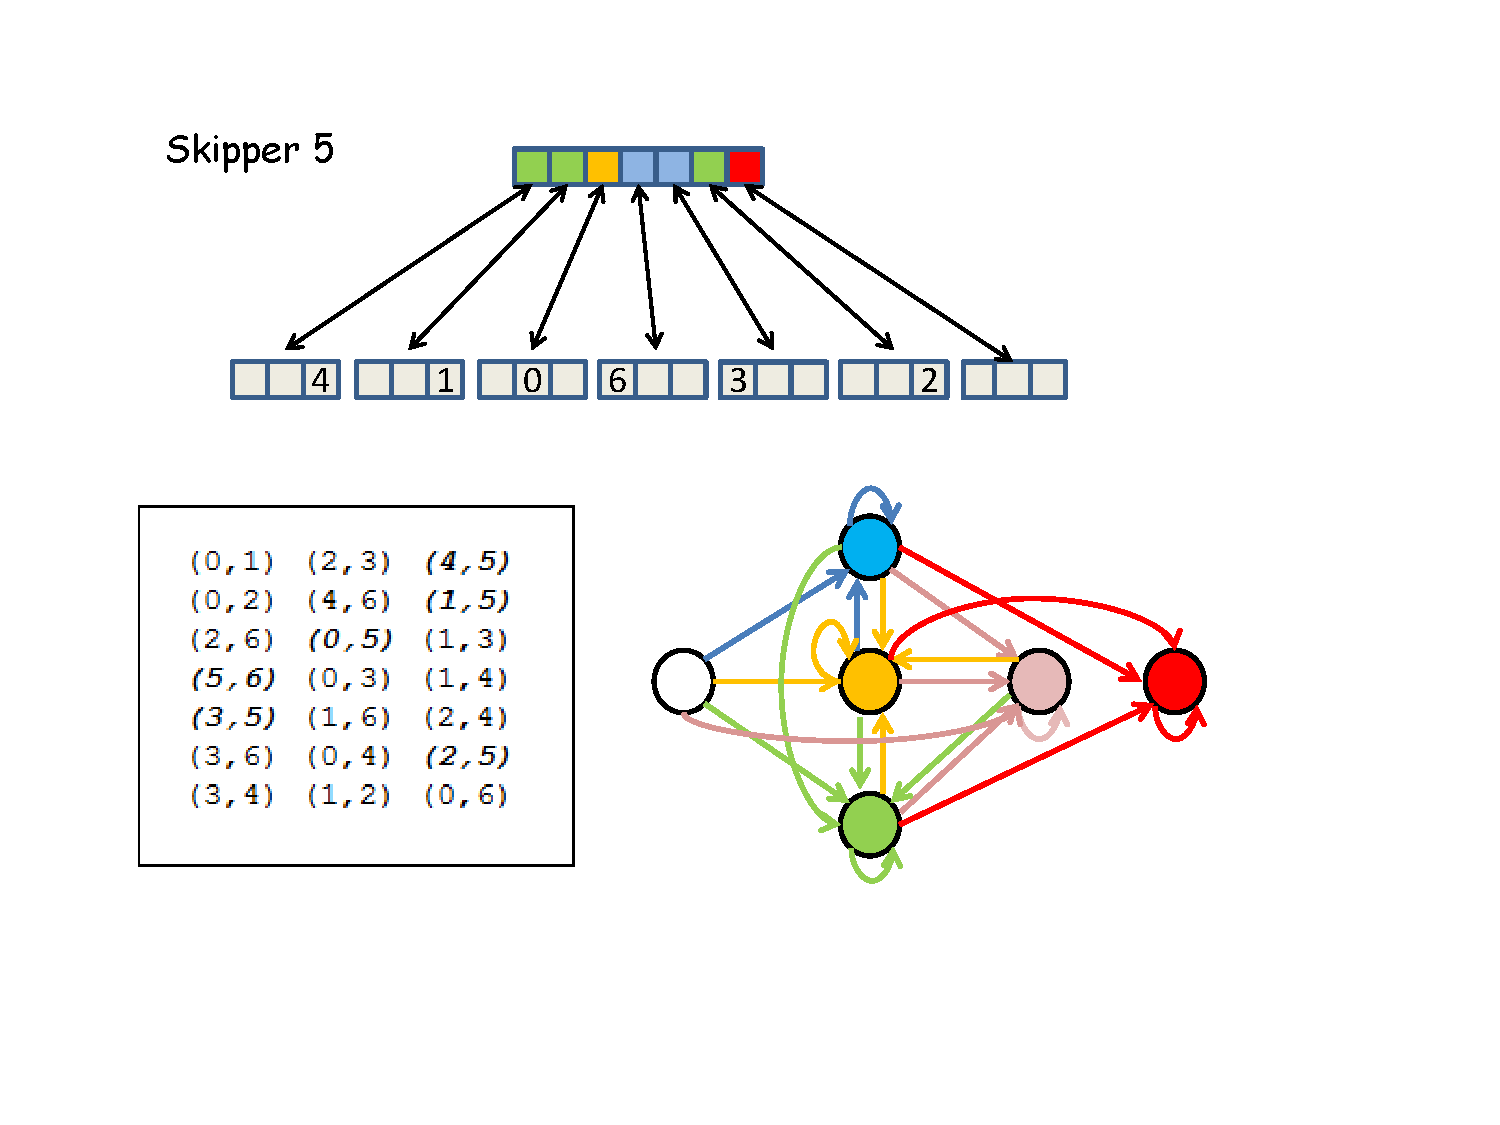
\includegraphics[height=10.2cm,width=13.2cm]{skipper5.pdf}
\vspace{-25mm}
\caption{A pictorial representation of a skipper (skipper 5) with multicoloured state and grey timeslots. The schedule for skipper 5 is in bold and the deterministic finite automata for criteria 4, 11 and 12 is drawn with state $\START$ in white, $\FIRST$ in blue, $\MID$ in yellow, $\LAST$ in green, $\BYE$ in pink and $\END$ in red.}
\label{skipper5}
\end{figure}

\noindent
We are now in a position to model criteria 1 (each skipper sails against every other skipper) and optimisation criteria 10 (minimise boat changes).  In (\ref{eq13}), (\ref{eq14})  and (\ref{eq15}) we present a
match-perspective of the schedule, using a two dimensional array of variables $\match$, where $\match[{i,j}]$ is the time slot that skippers $s[{i}]$ and $s[{j}]$ meet in a match. Only the half above the diagonal is represented and the lower half is made up of exactly the same variables, i.e. $\match[{i,j}]$ is \emph{exactly} the same constrained variable as $\match[{j,i}]$.  Constraint (\ref{eq15}) states that  a match between skippers $s[{i}]$ and $s[{j}]$ takes place at time $k$ (i.e. $\match[{i,j}] = k$) if and only if  skipper $s[{i}]$'s $k^{th}$ time slot is skipper $s[{j}]$ and conversely that skipper $s[{j}]$'s $k^{th}$ time slot is skipper $s[{i}]$.  Constraints (\ref{eq16}), (\ref{eq17})  and (\ref{eq18}) then convert this from time slots to flights, i.e. $\modMatch[{i,j}]$ is the flight in which skippers $s[{i}]$ and $s[{j}]$ meet for a match. Finally, constraint (\ref{eq19}) ensures that each skipper's match occurs in different flights. Also, since $\modMatch[{i,j}] \equiv \modMatch[{j,i}]$, setting rows to be all different also ensures that columns are all different.

%
% the match array
%
\begin{flalign}
    & \forall_{i \in [0..n-2]} ~ \forall_{j \in [i+1..n-1]}  ~\match[{i,j}] \in \{0..t-1\} \label{eq13} \\
    & \forall_{i \in [0..n-2]} ~ \forall_{j \in [i+1..n-1]}  ~\match[{j,i}] \equiv \match[{i,j}] \label{eq14} \\
    & \forall_{i \in [0..n-2]} ~ \forall_{j \in [i+1..n-1]}  ~ \forall_{k \in [0..t-1]} ~ \match[{i,j}] = k \iff s[{i}].\timeSlot[{k}] = j  ~ \wedge ~ s[{j}].\timeSlot[{k}] = i  \label{eq15} \\
    & \forall_{i \in [0..n-2]} ~ \forall_{j \in [i+1..n-1]}  ~ \modMatch[{i,j}] \in \{0..f-1\} \label{eq16} \\
    & \forall_{i \in [0..n-2]} ~ \forall_{j \in [i+1..n-1]}  ~ \modMatch[{j,i}] \equiv \modMatch[{i,j}] \label{eq17} \\
    & \forall_{i \in [0..n-2]} ~ \forall_{j \in [i+1..n-1]}  ~ \modMatch[{i,j}] = \frac{\match[{i,j}]}{m} \label{eq18} \\
    & \forall_{i \in [0..n-1]} ~ \allDifferent(\modMatch[{i}]) \label{eq19}
\end{flalign}

\noindent
We now take a temporal view (\ref{eq20}), such that $time[{\tau}]$ is a pair $(i,j)$, stating that at time $\tau$ skippers $s[{i}]$ and $s[{j}]$ are in a match, i.e. we channel between the match-perspective and the temporal-perspective.
%
% one dimensional time and decision variables
%
\begin{flalign}
    & \forall_{\tau \in [0..t-1]} ~ time[{\tau}] \in \{(0,1) .. (n-2,n-1)\} \label{eq20} \\
    & \forall_{\tau \in [0 .. t-1]} ~ \forall_{i \in [0..n-2]} ~ \forall_{j \in [i+1..n-1]}  ~ time[{\tau}] = (i,j) \iff \match[{i,j}] = \tau \label{eq21}
\end{flalign}

\noindent
Finally we have the optimisation criteria (criteria 10) to minimise the number of boat changes. This is presented in (\ref{eq22}) and (\ref{eq23}) below.

%
% optimisation criteria 10
%
\begin{flalign}
    & \totalBoatChanges = \sum_{i=0}^{n-1} s[{i}].\totalChange  \label{eq22} \\
& minimise(\totalBoatChanges) \label{eq23}
\end{flalign}

Figure \ref{schedChanges} gives a pictorial view of the model, using the 7 skipper and 6 boat problem. On the right we have the 7 skippers with their states and time slots. Again, top right, we give the schedule actually produced.  Middle left we have the $\match$ array and at the bottom the $time$ array. Above the $match$ array we have the $\modMatch$ array. The yellow arrows show the channeling between parts of the model.

\begin{figure}[h]
\centering
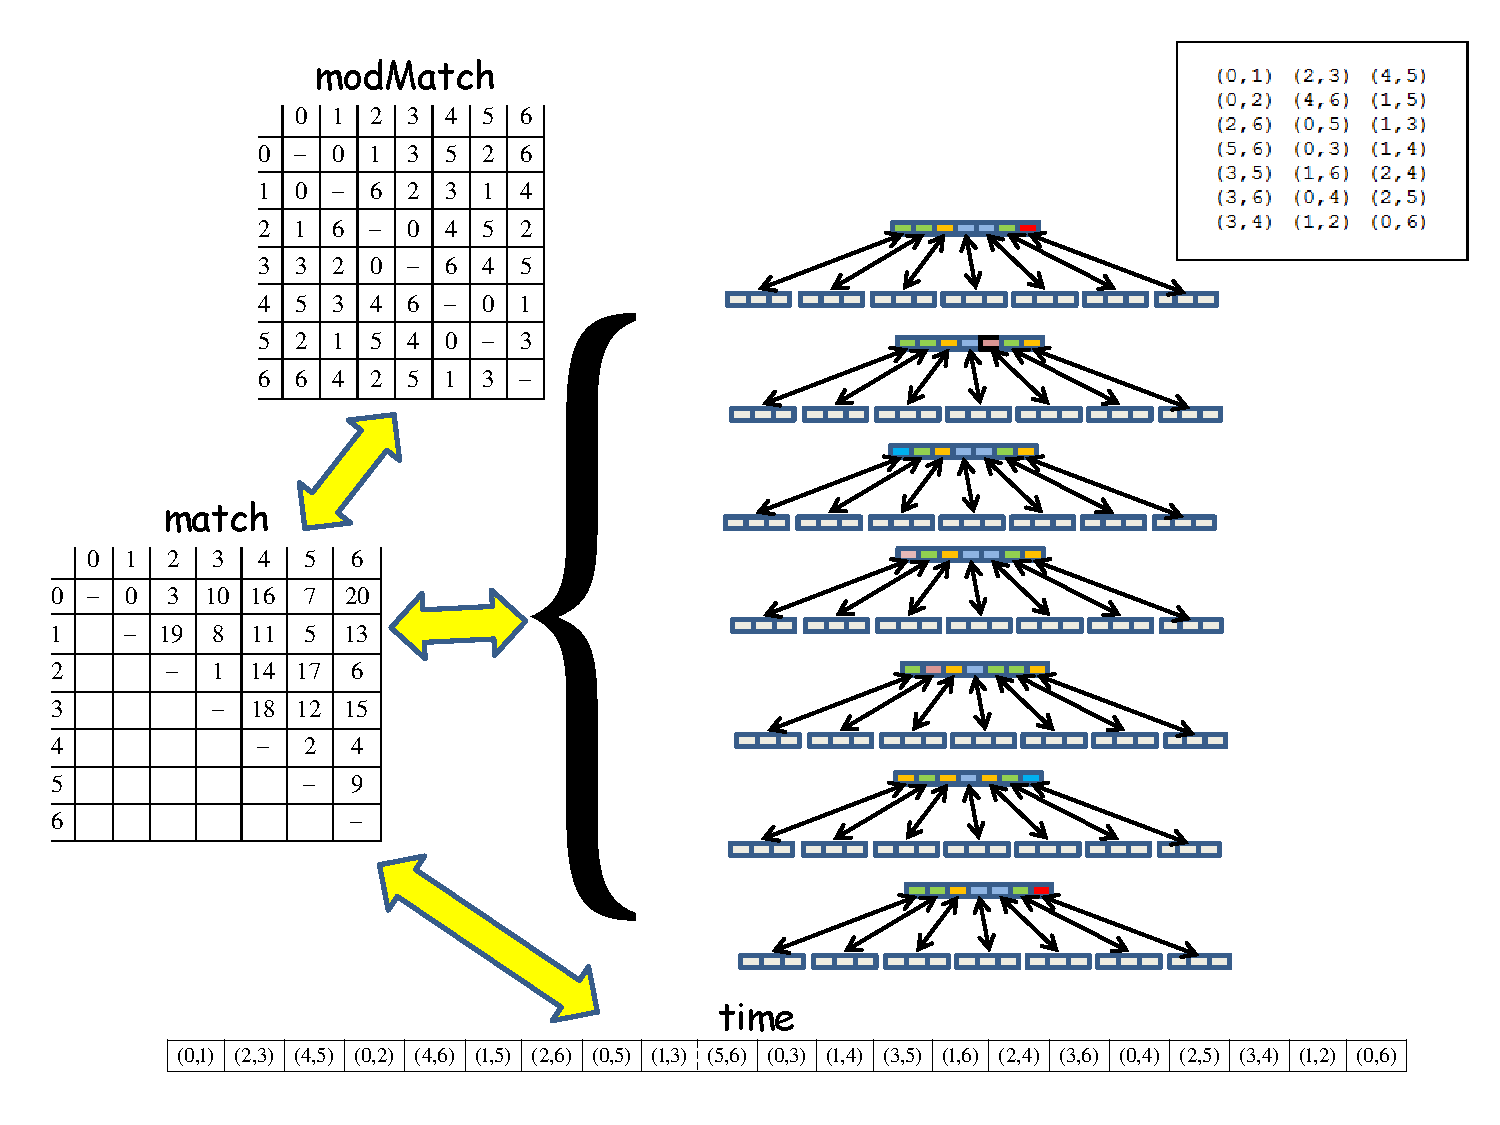
\includegraphics[height=10.2cm,width=13.2cm]{schedule.pdf}
%\vspace{-35mm}
\caption{A pictorial representation of the entire model of the schedule for 7 skippers and 6 boats. The schedule is reproduced top right. On the right we have the 7 skippers, on top left the $\modMatch$ array, at the bottom $time$ and middle left the $\match$ array. The yellow arrows signify channeling between parts of the model.}
\label{schedChanges} 
\end{figure}

The decision variables are $time[{0}]$ to $time[{t-1}]$, i.e. for each time slot we decide what match takes place. A symmetry break is made at the top of search by forcing the first round to contain the matches (0,1), (2,3), ... i.e. $\forall_{i \in [0..m-1]} ~ \match[{2.i,2i+1}] = i$. The schedule presented has 6 boat changes: there are no boat changes in flight 0 (first flight), flight 1 skipper 6 has a boat change, flight 2 skipper 3 has a boat change, flight 3 it's skipper 4, flight 4 skipper 6, flight 5 skipper 0 and last flight skipper 1.

\subsection{Stage 2 and 3: minimising imbalance and renaming skippers}
Having produced a schedule that minimises boat changes, we then minimise criteria 6, imbalance. Assuming the first stage produced a schedule with $\beta$ boat changes we post this as a hard constraint in stage 2, i.e. $\totalBoatChanges \leq \beta$. For each skipper $\sigma$ we introduce a zero/one variable $position[{i,j}]$  (\ref{posA}) which is 1 if and only if skipper $\sigma$ is in a match in time $m.j + i$, i.e. in the $i^{th}$ match of the  $j^{th}$ flight (\ref{posB}). Imbalance is then computed via (\ref{imbA}) for each position, as the absolute amount of over or under expected presence in a given postion. Finally, (\ref{imbB}) we compute the maximum imbalance over all positions for this skipper.

\begin{flalign}
    & \forall_{i\in [0..m-1]} ~ \forall_{j \in [0..f-1]} ~ \sigma.\position[{i,j}] \in \{0,1\} \label{posA} \\
    & \forall_{i \in [0..m-1]} ~ \forall_{j \in [0..f-1]} ~ \sigma.\position[{i,j}] = 1 \iff \sigma.\timeSlot[{m.j+i}] \geq 0 \label{posB} \\
    & \forall_{i \in [0..m-1]} ~ \imbalance[{i}] = |\frac{n-1}{m} - \sum_{j=0}^{f-1} \position[{i,j}]| \label{imbA} \\
& \sigma.\maxImbalance = \sigma.maximum(\sigma.imbalance)  \label{imbB}
\end{flalign}

\noindent
We then capture the maxmum imbalance over all skippers (\ref{balAllA} and \ref{balAllB}) and minimise this (\ref{balAllC}). As before, the decision variables are $time[{0}]$ to $time[{t-1}]$ and the same symmetry breaking is imposed at top of search.

\begin{flalign}
    & \forall_{i \in [0..n-1]} ~ \imbalance[{i}] = \sigma[{i}].\maxImbalance \label{balAllA} \\
& \maxImbalance = maximum(\imbalance) \label{balAllB} \\
& minimise(\maxImbalance) \label{balAllC}
\end{flalign}

\noindent
Stage 3 then takes as input the schedule produced in stage 2 and renames skippers in the last round of the last flight to be (0,1), satisfying criteria 9. This is a simple linear process. The schedule produced for 7 skippers and 6 boats is shown in Table \ref{tab2}.

\begin{table}[h]
%\vspace{-0.2cm}
\begin{center}
\begin{tabular}{cc} \\ 
flight & matches \\ \hline
0 & (0,6) (2,3) (4,5) \\
1 & (0,2) (4,1) (6,5) \\
2 & (2,1) (0,5) (6,3) \\
3 & (5,1) (0,3) (6,4) \\
4 & (3,5) (6,1) (2,4) \\
5 & (3,1) (0,4) (2,5) \\
6 & (3,4) (6,2) (0,1) \\ \hline
\end{tabular}
\end{center}
\caption{Round-robin schedule with 7 skippers, 6 boats and 7 flights. Result of stages 1, 2, and 3. It has 6 boat changes and imbalance 1. An example of imbalance is skipper $\sigma[{0}]$ with 2 matches in position 0 (first), 3 in position 1 and 1 (mid) in position 2 (last). Perfect balance would be 2 matches in each position, only achieved by skipper 2.}
\label{tab2}
\end{table}

\subsection{Stage 4: orienting matches}
The final stage, stage 4, orients skippers within matches, such that they are either port (red) or starboard (green). This is done to satisfy criteria 2 and 3, 5 and 8. A sketch of the constraint model is given with a supporting diagram, Figure \ref{oriented}.  A sequence of zero/one constrained integer variables, of length $n-1$, is produced for each skipper. These correspond to the sequence of skippers they meet in matches. For example, taking the schedule in Table \ref{tab2}, skipper $\sigma[{2}]$ meets skippers in the following order: 3,0,1,4,5,6 and skipper $\sigma[{5}]$ in the order: 4,6,0,1,3,2. Therefore, skipper $\sigma[{2}]$'s 4$^{th}$ variable must take a different value from $\sigma[{5}]$ 5$^{th}$ variable. There are summation constraints on each skipper to enforce criteria 2 and 3 (equal number of port and starboard matches). Criteria 8 is enforced by posting constraints such that in a match ($\sigma[{i}],\sigma[{j}]$) where $|i - j| = 1$ the higher indexed skipper (lower ranked) is on the port side. A deterministic finite automata constraint is posted for criteria 5 (restricting sequences of port and starboard assignments). 

In Figure \ref{oriented} port is red and starboard green. The sequence of zero/one variables for each skipper is shown on the left. Bottom right is the dfa, and top right is the final schedule produced from stages 1 to 4. The schedule has 6 boat changes and a maximum imbalance of 1. Three days cpu time was devoted to stages 1 and 2. Stages 3 and 4 completed in 15 milliseconds. The schedule presented here is new, not appearing in the ISAF World Sailing Umpire's Manual.
\begin{figure}[h]
\centering
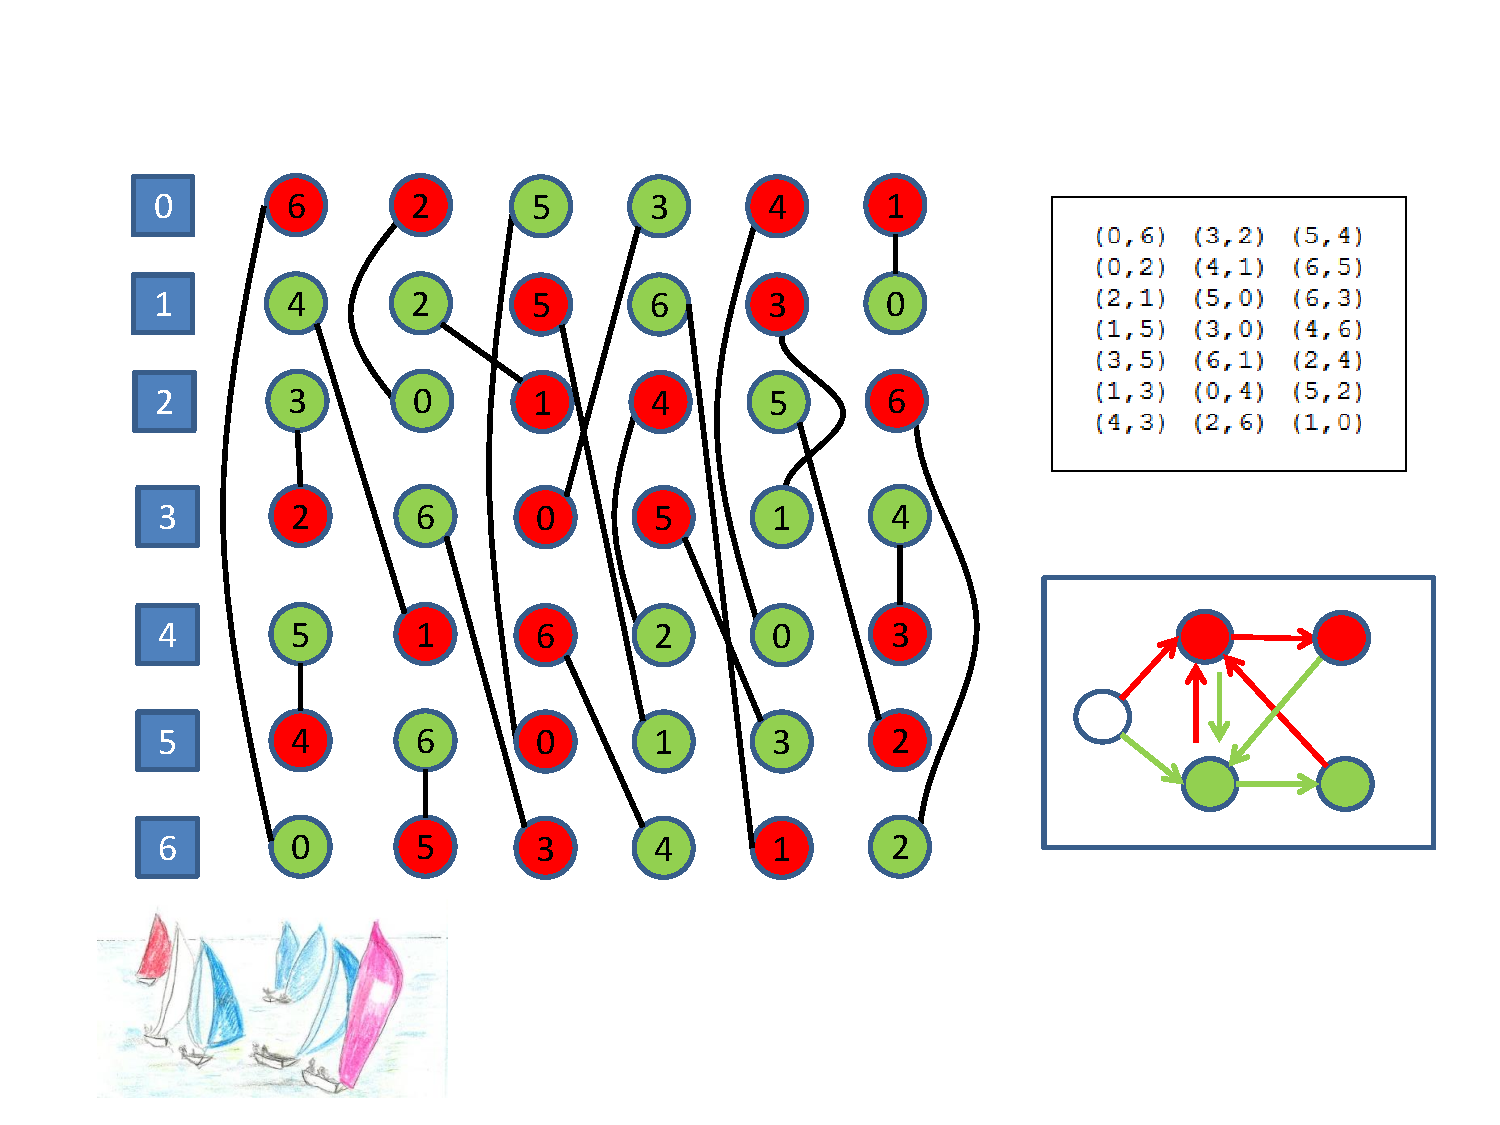
\includegraphics[height=10.2cm,width=13.2cm]{oriented.pdf}
%\vspace{-35mm}
\caption{A pictorial representation of the orientation process, stage 4. Top right is the actual oriented schedule. Below that is the dfa to satisfy criteria 5. On the left is the zero/one variables, a row representing a skippers sequence of competitors. An edge between variables corresponds to a matched pair, that must take different values. Bottom right is a sketch by one of the authors.}
\label{oriented} 
\end{figure}

\section{Sample Schedules}

\subsection{Discussion}

\section{Conclusion}

\section*{Acknowledgments}
We would like to thank our parents, God and all his angels.
\coffee{2}

\bibliographystyle{plain}
\bibliography{bib}

\end{document}
